\chapter{Techniques de collecte d'informations}
\label{chap:Mini Projet}
Lors du début de chaque CTF ou de pentesting en général, il y a une phase très importante qu'il ne faut pas oublier qui est la recherche d'informations sur la machine à attaquer. Il existe 2 types de recherche d'informations :

\begin{itemize}
  \item Collecte d'informations passive
  \item Collecte d'informations active 
\end{itemize}

 Nous verrons dans un premier temps la collecte d'informations passive d'une cible puis la collecte d'informations active.

\section{Collecte d'informations passive}

La collecte d'informations passive est le moyen par lequel un attaquant peut récupérer des informations sur une entreprise ou une machine, sans entrer directement en contact avec cette dernière. En effet, ces informations sont la plupart du temps trouvable sur internet.

Par exemple, à partir de recherches sur internet, on peut trouver des adresses IP ou encore des emails ou des noms de domaines. Toutes ces informations peuvent être d'ordre publique. Une simple commande \lstinline{ping} sur un site internet permet de récupérer une adresse IP. Imaginez par exemple, une attaque contre \url{http://rt.iut-velizy.uvsq.fr/}. Il va falloir dans un premier temps déterminer quels systèmes sont utilisés par la société et quels sont les systèmes que nous pouvons attaquer. De plus, certains systèmes peuvent ne pas appartenir à la société cible et pourraient alors être considérés comme hors de portée de l'attaque.

\subsection{Whois}

Whois ("Qui est" en francais)  est un outil permettant d'interroger des bases d'informations (registres) concernant les noms de domaines et adresses IP. Les données contenues dans ces bases ne comportent aucune forme de garantie mais permettent généralement de retrouver le propriétaire d'un domaine ou d'une machine.

 Il existe plusieurs bases de données connues:

\begin{itemize}
    \item RIPE NCC (Réseaux IP Européens, whois.ripe.net) pour l'Europe
    \item APNIC (Asia Pacific Network Information Center) pour l'Asie et le Pacifique
    \item ARIN (American Registry for Internet Numbers, whois.arin.net) pour l'Amérique du Nord et l'Afrique Sub-Saharienne
    \item LACNIC (Regional Latin-American and Caribbean IP Address Registry, whois.lacnic.net) pour l'Amérique latine et les Caraïbes
    \item  INTERNIC (whois.internic.net) pour les autres parties du globe
\end{itemize}

 Il existe des sites sur internet permettant d'utiliser cet outil. Il est également présent sous Kali linux.\\

 \textbf{Utilisation de la commande whois avec Kali linux:}\\
Nous allons utiliser whois sur le site \url{uvsq.fr} dans \textbf{figure \ref{fig:whois}}.\\

\begin{figure}[htp!]
  \centering
  \setlength\figureheight{7cm}
  \setlength\figurewidth{9cm}
  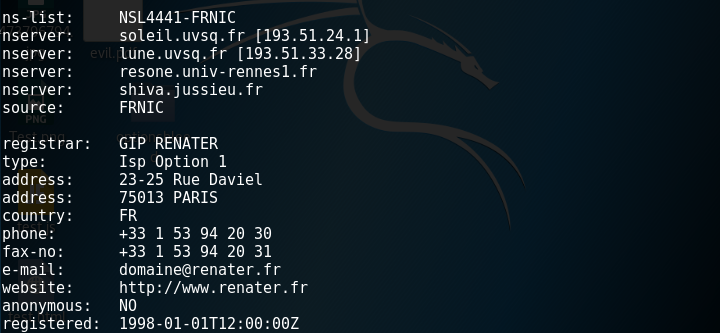
\includegraphics[width=1\textwidth]{oui/images/Whois/whois2.PNG}
  \caption{whois uvsq.fr}
  \label{fig:whois}
\end{figure}

 La commande whois nous donne des informations sur le nom de domaine \url{uvsq.fr}. On apprend ici les différents serveurs DNS qui gèrent ce domaine dans la  \textbf{figure \ref{fig:whoisdns}}.

\begin{figure}[htp!]
  \centering
  \setlength\figureheight{7cm}
  \setlength\figurewidth{9cm}
  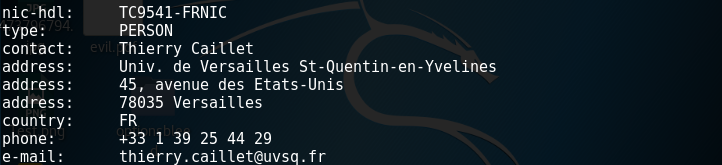
\includegraphics[width=1\textwidth]{oui/images/Whois/whois3.PNG}
  \caption{whois uvsq.fr}
  \label{fig:whoisdns}
\end{figure}

 Whois est capable de récupérer l'email de l'administateur qui gère le domaine \url{uvsq.fr}. Ces informations peuvent être plus ou moins utiles lors d'une attaque.

Il est également possible de spécifier l'adresse IP de \url{www.uvsq.fr} pour récupérer des informations relatives à l'adresse IP comme vous pouvez voir en \textbf{figure \ref{fig:whoisip}}.

\begin{figure}[b!]
  \centering
  \setlength\figureheight{7cm}
  \setlength\figurewidth{9cm}
  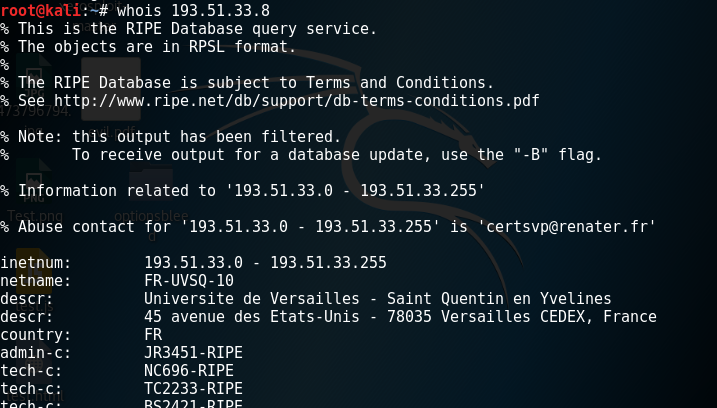
\includegraphics[width=0.9\textwidth]{oui/images/Whois/whois4.PNG}
  \caption{whois ip www.uvsq.fr}
  \label{fig:whoisip}
\end{figure}
%parler du champ inetnum et qu'on a la range d'IP pour uvsq.fr https://www.apnic.net/manage-ip/using-whois/guide/inetnum/ https://www.ripe.net/manage-ips-and-asns/db/support/documentation/ripe-database-documentation/rpsl-object-types/4-2-descriptions-of-primary-objects/4-2-4-description-of-the-inetnum-object
 --- Le champ \textbf{inetnum} correspond à une plage d'adresse IP détenue par le domaine en question. Par exemple, pour le domaine \url{uvsq.fr} sa plage d'IP sera comprise entre \textbf{193.51.33.0} et \textbf{193.51.33.255}.\\

Un simple script en python permet de vérifer cela et d'obtenir un résultat visible en \textbf{figure \ref{fig:resultatprogpy}}.  (Script en annexe \ref{fig:nslookup})

\begin{figure}[b!]
  \centering
  \setlength\figureheight{7cm}
  \setlength\figurewidth{9cm}
  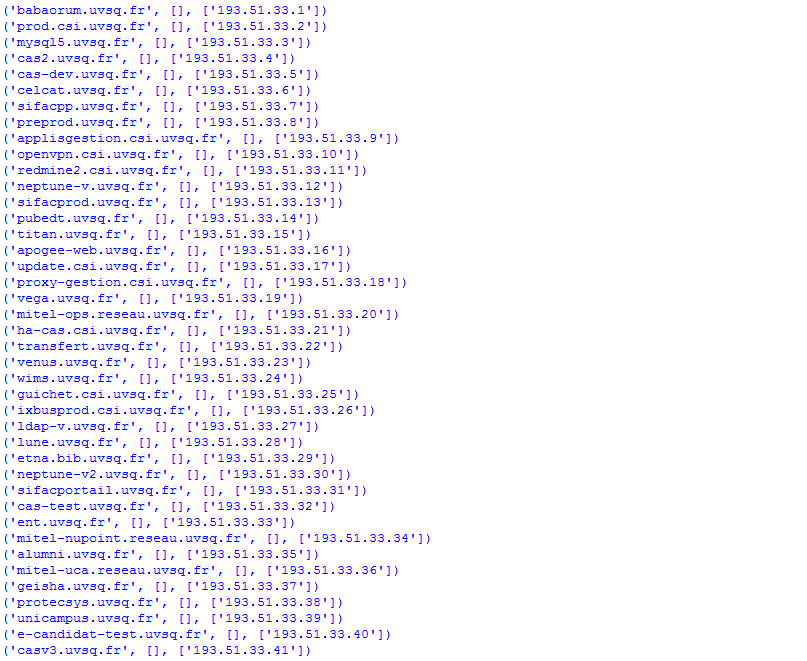
\includegraphics[width=0.8\textwidth]{oui/images/Whois/script-python.PNG}
  \caption{Résolution DNS pour la plage d'ip de uvsq.com}
  \label{fig:resultatprogpy}
\end{figure}

 On constate à travers cette capture que les IP de la plage pointent vers le nom de domaine \url{uvsq.fr}. Cela peut être très utile pour cibler des services à attaquer avec leur IP public. Par exemple, l'IP \textbf{193.51.33.3} semble correspondre à un potentiel serveur mysql à en croire son nom. On remarque également que l'autorité de \textbf{uvsq.com} a créé un alias de l'enregistrement \textbf{www} vers \textbf{preprod.uvsq.com}, puisque ces noms ont les même IP et qu'ils redirigent tous deux vers le site internet de l'uvsq.\\

 --- Le champ \textbf{netname} correspond au nom donné à une plage d'adresses IP. Un nom de réseau est composé de lettres, de chiffres, du caractère de soulignement et du trait d'union. Le premier caractère d'un nom doit être une lettre, et le dernier caractère d'un nom doit être une lettre ou un chiffre.\\

\subsection{Nslookup}

L'outil Nslookup est un outil implanté sur beaucoup de systèmes d'exploitation (OS) tel que Windows ou Linux. Cet outil permet de faire des résolutions DNS à partir d'un nom de domaine. En effet, cela est très pratique lorsqu'on veut récupérer une IP à partir d'un nom tel que \textbf{www.uvsq.fr}.\\

 \textbf{Fonctionnement requête DNS}\\

Nous allons ici présenter le bref fonctionnement d'une requête DNS puisque cette partie a déjà été expliqué dans d'autres modules auparavant. En premier lieu, le DNS permet d'associer un nom à une IP ce qui est très utile pour l'être humain.\\

 Le protocole DNS est un protocole UDP avec comme numéro de port 53. Le DNS est un modèle réparti hiérarchisé, sa mise en œuvre requiert plusieurs serveurs qui prennent en charge individuellement la traduction de parties complémentaires de l’espace des noms afin de rendre plus souple le traitement des sollicitations. Ces parties appelées "zones" sont en fait des domaines de noms dont l’administration est définie et attribuée à un ou plusieurs serveurs.

 La \textbf{figure \ref{fig:repartitiondns}} nous présente un schéma de la répartition des zones DNS.

\begin{figure}[htp!]
  \centering
  \setlength\figureheight{7cm}
  \setlength\figurewidth{9cm}
  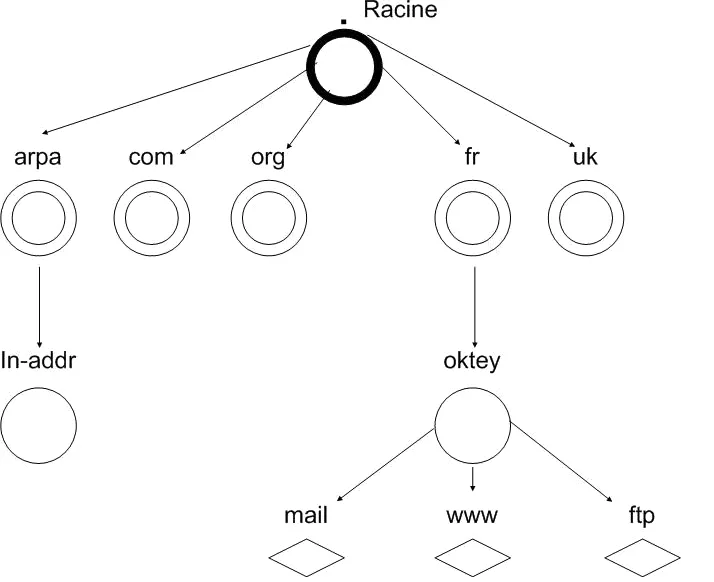
\includegraphics[width=0.5\textwidth]{oui/images/Nslookup/dns.png}
  \caption{Répartition des zones DNS}
  \label{fig:repartitiondns}
\end{figure}

 Le domaine Racine est géré par les 13 serveurs DNS nommés \lstinline{<x>.root-servers.net}, où \lstinline{<x>} est une lettre comprise entre ‘a’ à ‘m’. Ces serveurs racines sont gérés par des organisations différentes nommées par l’ICANN. Les domaines enfants sont dits les domaines de premier niveau ou TLD (Top Level Domain). On y retrouve le domaine .com, .fr etc...\\

\newpage

Expliquons maintenant ce qu'il se passe lorsqu'un client effectue une requête DNS.

Il existe deux types de requête DNS. Les requêtes itératives, et récursives. Nous ne présenterons ici que les requêtes récursives, comme illustré sur la \textbf{figure \ref{fig:dns2}}.

\begin{figure}[t]
  \centering
  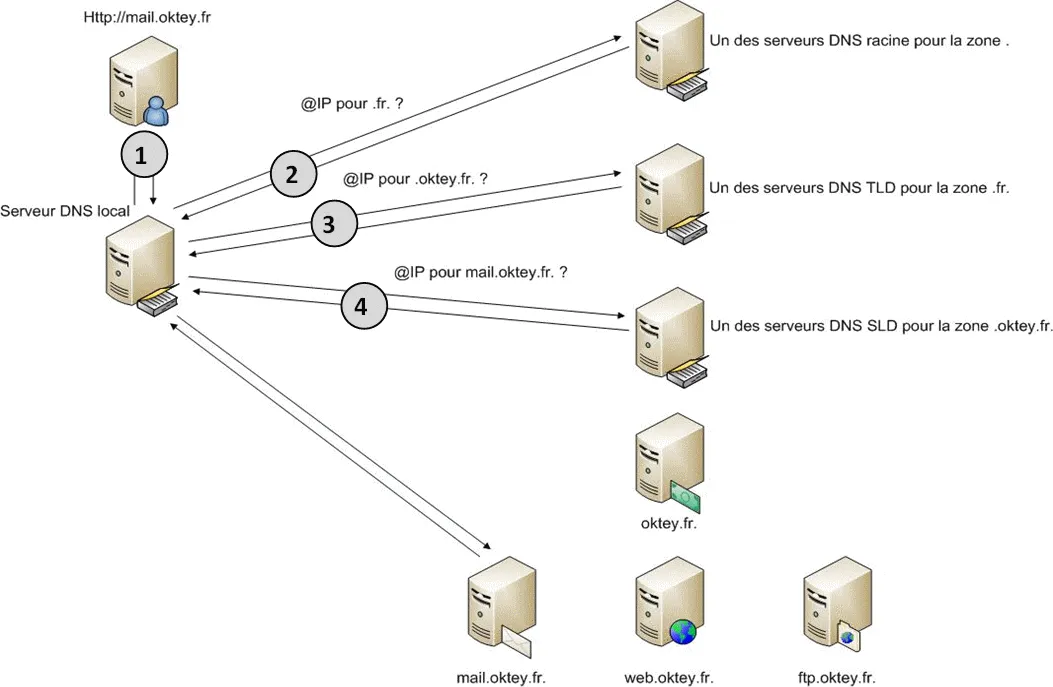
\includegraphics[width=0.6\textwidth]{oui/images/Nslookup/dns2.png}
  \caption{Schéma d'une requête DNS récursive}
  \label{fig:dns2}
\end{figure}

\begin{enumerate}
    \item Le client effectue une requête DNS à son serveur DNS local.
    \item Le serveur DNS contacte le serveur racine pour récupérer l'ip du serveur TLD de la zone fr.
    \item Le DNS local contacte le TLD de la zone fr pour récupérer l'ip du sous domaine oktey.
    \item Ce dernier contacte le serveur qui fait autorité sur la zone oktey.fr pour récupérer l'ip associé à l'enregistrement mx de mail.okley.fr.
\end{enumerate}

 On constate qu'avec l'utilisation des requête récursives, c'est le serveur DNS local qui s'occupe de faire toutes les requêtes.\\
 Avec l'outil \textbf{Nslookup}, il est également possible d'effectuer une résolution inverse. En effet, cette dernière permet de récupérer le nom associé à une adresse IP. Pour ce faire, on utilise le domaine \textbf{in-addr.arpa} (RFC 1035) pour retrouver le nom associé.

 La technique de résolution inverse a été utilisée dans la figure 2.4. En effet, à partir de la plage d'IP récupéré avec l'outil \textbf{whois}, on peut effectuer des résolutions inverses pour tenter de récupérer le nom derrière ces IP. Ainsi, cela peut nous indiquer un service qui serait hébergé par cette IP. A partir de là, il sera plus facile d'orienter nos recherches pour continuer l'attaque.


\subsection{Maltego}

Maltego est un outil open source intélligent permettant la recherche d'informations précises sur une personne ou une entreprise. On appel ce genre d'outil un footprinting (reconnaissance passive). Maltego permet l'automtisation des tâches de recherches. Ainsi, avec ces informations, Maltego les représentent sous forme d'un graphique détaillé.\\

\begin{figure}[htp!]
  \centering
  \setlength\figureheight{7cm}
  \setlength\figurewidth{9cm}
  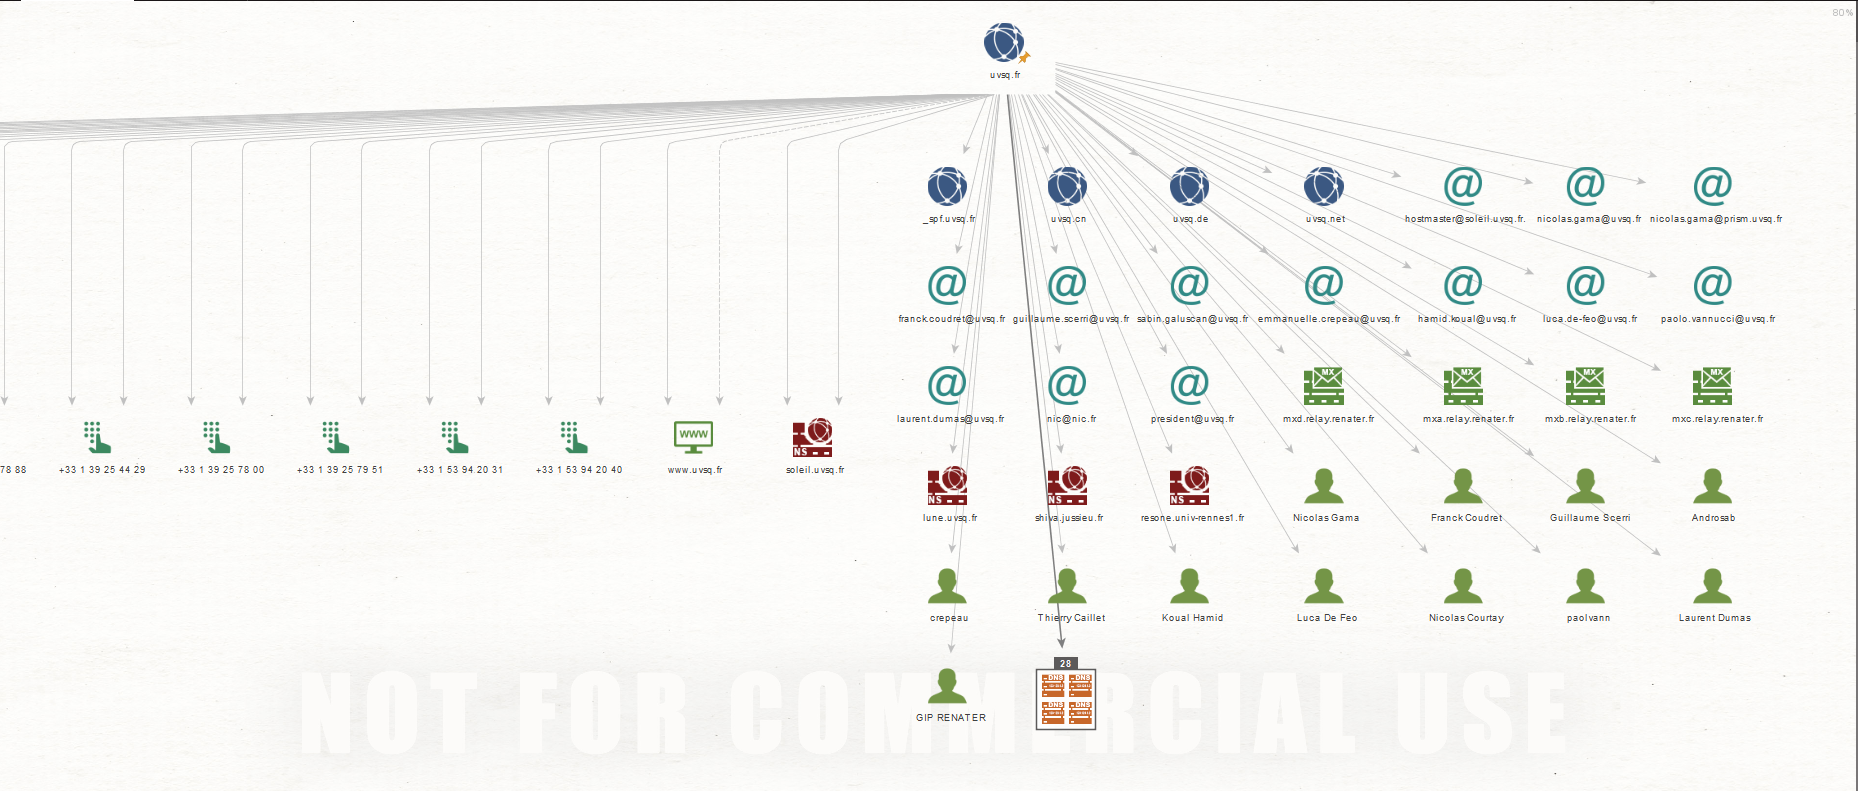
\includegraphics[width=1\textwidth]{oui/images/maltego/uvsq2.PNG}
  \caption{Présentation graphique de maltego}
  \label{fig:graphmaltego}
\end{figure}

\newpage
Dans la \textbf{figure \ref{fig:graphmaltego}}, on peut voir l'utilisation de Maltego sur le domaine \textbf{uvsq.com}. On peut donc récupérer des adresses mails, des numéros de téléphone, des noms de personnes ainsi que les sous domaines DNS associés à \textbf{uvsq.com}. Il est également possible de récupérer des adresses IP ainsi que le numéro d'AS sur lequel le site est hébergé.\\

Pour fonctionner, Maltego travaille à partir de bases de données ainsi que de recherches faites sur le web. En somme, cela évite à l'utilisateur de faire de longues recherches pour trouver une information sur une personne ou un site. Cela peut être extrêmement utile lors de la collecte d'informations sur une entreprise. En effet, avec les informations que nous pouvons récupérer, il serait possible de cibler plus facilement les attaques ou même de faire du phishing avec les adresses emails obtenues.
%

\newpage
\section{Collecte d'informations active}

La collecte d'informations active va consister à reccueillir des informations en effectuant des requêtes sur le réseau et/ou machine cible. Cette étape va donc nous permettre de récupérer des informations telles que l'IP, l'adresse MAC, les ports ouverts, etc... Sans cette phase, une attaque serait impossible. C'est pourquoi il est important de penser à marquer dans un fichier texte l'ensemble des informations obtenues au cours de cette recherche. Nous allons dans cette partie vous présenter les outils adéquats et leur fonctionnement afin que vous puissiez obtenir facilement les données que nous pourrons exploiter par la suite. Nous verrons les outils suivants :

\begin{itemize}
    \item Arp-scan en tant que scanneur de machines
    \item Nmap en tant que scanneur de ports
    \item Dirb / Dirbuster en tant que scanneur de répertoire Web
    \item Nikto en tant que scanneur de vulnérabilités
\end{itemize}

\subsection{Arp-scan}

Arp-scan est un utilitaire qui permet  d’obtenir les adresses IP d’un réseau via la couche 2 du modèle OSI . Le modèle OSI est une norme d’exemple pour tous les types de transmissions réseaux. Ce modèle peut être vu comme en \textbf{figure \ref{fig:osi}}.
%Image modèle OSI
\begin{figure}[htp!]
  \centering
  \setlength\figureheight{7cm}
  \setlength\figurewidth{9cm}
  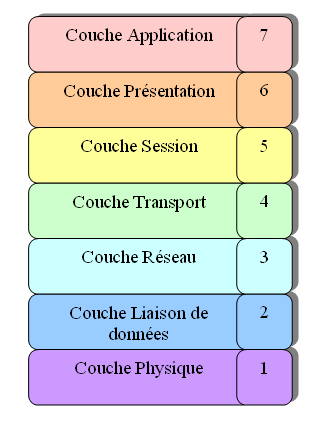
\includegraphics[width=0.4\textwidth]{oui/images/Arpscan/modeleOSI.PNG}
  \caption{Schéma du modèle OSI}
  \label{fig:osi}
\end{figure}

La couche 2 est la couche de liaison de données. Cette dernière correspond à l’adressage physique des machines, soit l’adresse MAC. L’adresse MAC est l’adresse unique d’une interface réseau d’un équipement. Cette adresse est codée en hexadécimal en 6 octets.\\

 \textbf{Fonctionnement d'Arp-scan}\\

Cet outil va envoyer une requête ARP en broadcast sur le réseau et afficher l’IP, l'adresse MAC ainsi que, si possible, l'origine de chaque hôte. Si un hôte ne répond pas, le paquet ARP sera envoyé à nouveau. Le nombre maximum de tentatives peut être modifié avec l'option --retry. Cependant, si l'on réduit le nombre de tentatives, alors cela réduira le temps du scan mais engendrera le risque de perdre certains résultats en raison de la perte de paquets.
Comme vous pouvez le voir sur la \textbf{figure \ref{fig:arpscanwireshark}}, la capture Wireshark effectuée après un "arp-scan" se présente de la même manière qu’une requête ARP.

%Image Wireshark arp broadcast
\begin{figure}[htp!]
  \centering
  \setlength\figureheight{7cm}
  \setlength\figurewidth{9cm}
  
\includegraphics[width=1\textwidth]{oui/images/Arpscan/wireshark.PNG}
  \caption{Capture Wireshark}
  \label{fig:arpscanwireshark}
\end{figure}

Le protocole ARP est un protocole de niveau 2 (couche de liaison de données) qui est utilisé pour déterminer l'adresse MAC (couche 2) d'un hôte distant à partir de son adresse IP (couche 3). Le protocole ARP a été conçu pour fonctionner avec n'importe quel format d'adresse de couche 2 et de couche 3, mais l'utilisation la plus courante est de cartographier un réseau.
Cependant, cet outil ne peut être utilisé que sur des réseaux LAN car les requêtes ARP ne peuvent pas être routées dans le cas d’un scan de réseau Local.
Ce protocole utilise des adresses IP, mais il n'est pas basé sur IP. Ainsi, Arp-scan peut être utilisé sur une interface qui n'est pas configurée pour IP. La \textbf{figure \ref{fig:arpscanl}} présente l'utilisation la plus commune de cet outil.

\begin{figure}[htp!]
  \centering
  \setlength\figureheight{7cm}
  \setlength\figurewidth{9cm}
  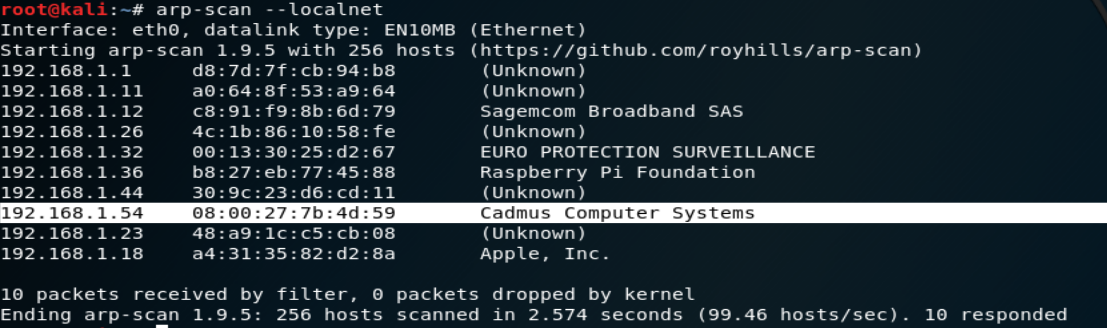
\includegraphics[width=0.9\textwidth]{oui/images/Arpscan/unknown.png}
  \caption{Arp-scan  - -localnet}
  \label{fig:arpscanl}
\end{figure}

Une fois l'IP cible récupérée, nous allons pouvoir analyser ses ports avec Nmap.

\subsection{Nmap}

Nmap est un utilitaire permettant de scanner les ports ouverts d’une machine ou d’un ensemble de machines présentes dans un même réseau. Les ports (logiciels) d'une machine permettent de distinguer les différents programmes qui écoutent et transmettent des informations sur cette machine. En effet, chaque programme ou service se verra atribuer un numéro de port qui servira à identifer le processus associé. En trouvant ces ports, Nmap se rend comme l’élément essentiel d’une attaque réseau. En effet, sans cette analyse, nous serions incapable de trouver un chemin d’attaque à moins d’avoir une chance inouïe. C’est pourquoi nous allons utiliser cet utilitaire pour résoudre nos CTFs.\\

 \textbf{Fonctionnement de Nmap}\\

Pour comprendre comment fonctionne Nmap, il va falloir revoir les bases du protocole TCP grâce à la \textbf{figure \ref{fig:3way}}.


\newpage

\begin{figure}[htp!]
  \centering
  \setlength\figureheight{7cm}
  \setlength\figurewidth{9cm}
  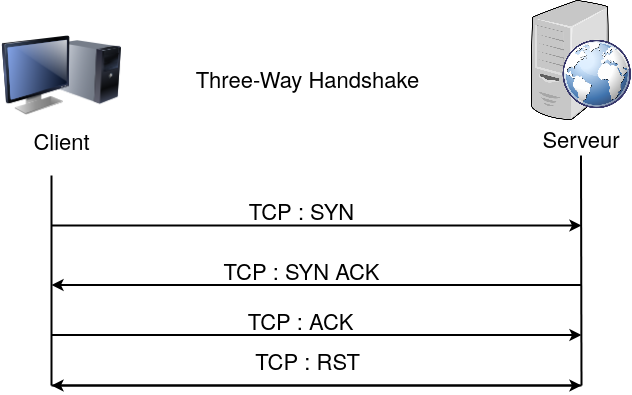
\includegraphics[width=0.8\textwidth]{oui/images/nmap/3way.png}
  \caption{Three-way Handshake}
  \label{fig:3way}
\end{figure}

Le protocole TCP de TCP-IP est situé au niveau de la couche Transport du modèle OSI (couche 4). Il va nous permettre d'établir une connexion fiable et sans pertes. Dans un premier temps, TCP va établir la connexion via le Three-way Handshake qui sont :

\begin{itemize}
    \item SYN
    \item SYN ACK
    \item ACK
\end{itemize}

A la suite de cette étape, le protocole de plus haut niveau faisant les requêtes pourra émettre et sera suivi dans un ACK TCP pour s'assurer de l'intégrité de la trame comme on peut le voir sur la \textbf{figure \ref{fig:acktcp}}.

\begin{figure}[htp!]
  \centering
  \setlength\figureheight{7cm}
  \setlength\figurewidth{9cm}
  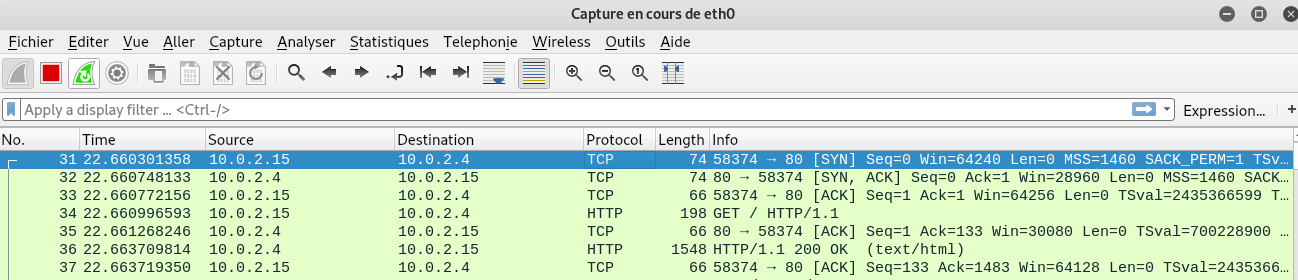
\includegraphics[width=1\textwidth]{oui/Ancien/imangeancien/Nikto/wireshark1.PNG}
  \caption{ACK TCP}
  \label{fig:acktcp}
\end{figure}

Sur l'exemple ci-dessus, on peut voir dans la section "Info" de Wireshark que les ports sont indiqués. On comprend alors que TCP ne cible pas une IP mais un socket. Un socket est l'ensemble de l'adresse IP et du port utilisé. Il est souvent représenté sous la forme suivante : \verb+192.168.1.200:80+. C'est donc en faisant varier le port du socket que Nmap pourra détecter si un port est ouvert ou non. Ainsi, si Nmap reçoit une réponse que de la machine cible à la suite d'un SYN TCP, cela voudra dire que le port est ouvert.\\
Maintenant que nous avons compris comment Nmap détecte si un port est ouvert ou non, nous allons nous intéresser à la détection du service associer à ce port. En effet, Nmap peut fournir le nom et même la version d'un service déployé sur un port d'une machine cible.\\

 Pour cela, l'outil se base sur deux fichiers qu'il utilise comme dictionnaire. Ces deux documents se situent dans son dossier d'éxécution et sur internet :

\begin{itemize}
    \item \textbf{nmap-services: https://svn.nmap.org/nmap/nmap-services}
    \item \textbf{nmap-services-probes: https://svn.nmap.org/nmap/nmap-service-probes}
\end{itemize}

 Le fichier nmap-services contient une association de nom de service en fonction du port. En effet, il existe trois catégories de ports :

\begin{itemize}
    \item \textbf{1-1023 : Well-known ports}
    \item \textbf{1024-49151 : Registered ports}
    \item \textbf{49152-65535 : Dynamic ports}
\end{itemize}

 Les "Well-kown ports" sont des ports attitrés à des service par l'IANA (Internet Assigned Numbers Authority). Ces services sont les plus connus du monde des réseaux et doivent être éxécutés en tant qu'administrateur. Les "Registered ports" sont eux aussi attribués par l'IANA mais ne nécessitent pas d'une éxecution en tant qu'administrateur. Les "Dynamic ports" ou ports dits "éphémères", comme le nom l'indique, sont distribués de manière dynamique par le système d'exploitation afin de pouvoir rentrer en contact avec un service. C'est donc en fontion de ce recensement que Nmap met à jour sa liste nmap-services. La question la plus légitime à la suite de cette explication est la suivante :\\
"Comment Nmap peut récupérer le nom d'un service déployé sur un port n'ayant pas été répertorié ?"\\
Nmap vous répondra en fonction de votre requête. En effet, si vous n'effectuez qu'un simple scan, l'outil ne va s'appuyer que sur nmap-services pour détecter le service. Cependant, si vous vous voulez avoir de plus amples informations sur le port, il vous faudra effectuer un scan de version. Ce scan se base sur le fichier "nmap-service-probes". Ce dernier contient des requêtes à effectuer en fonction des ports ouverts et des expressions régulières à tester avec la réponse du services. Si le test est positif, Nmap pourra afficher les informations présentes à la suite de l'expression régulière. Ce type de scan est donc beaucoup plus précis. La \textbf{figure \ref{fig:fonctionnementnmap}} représente donc le fonctionnement de base de Nmap.

\begin{figure}[htp!]
  \centering
  \setlength\figureheight{7cm}
  \setlength\figurewidth{9cm}
  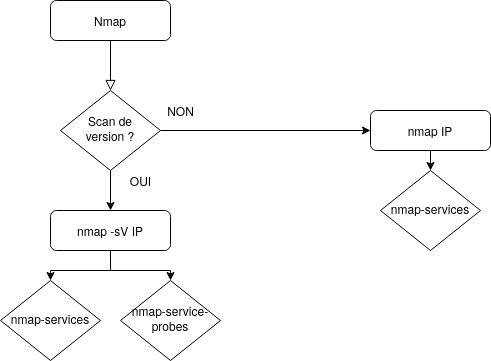
\includegraphics[width=0.9\textwidth]{oui/images/nmap/basenmapdiag.png}
  \caption{Schéma fonctionnement Nmap}
  \label{fig:fonctionnementnmap}
\end{figure}

Nous allons voir maintenant comment appliquer ce fonctionnement à un CTF.

 \textbf{Application de Nmap}\\

Dans cette partie, nous allons voir comment utiliser Nmap en ligne de commandes (CLI) en fonction des informations que l'on souhaite récupérer.\\

 \textbf{Mode basique}\\

Si vous souhaitez ne faire qu'un scan rapide sans option, la \textbf{figure \ref{fig:scanbasique}} présente la commande à effectuer.

\begin{figure}[htp!]
  \centering
  \setlength\figureheight{7cm}
  \setlength\figurewidth{9cm}
  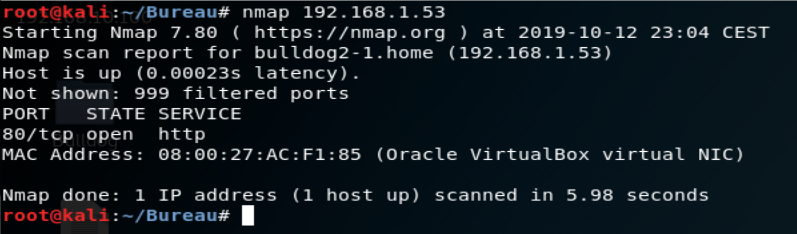
\includegraphics[width=0.7\textwidth]{oui/Ancien/imangeancien/Nmap/justeip.PNG}
  \caption{Scan basique}
  \label{fig:scanbasique}
\end{figure}

Comme on peut le voir ci-dessus, le résultat de ce scan simple nous permet de savoir que le port 80 est ouvert et que le sevice associé est HTTP. Si on observe un peu plus cette capture d'écran, on peut voir que Nmap a résolu via DNS le nom de notre cible qui est ici bulldog2-1.\\
Du côté de Wireshark, nous pouvons observer, en \textbf{figure \ref{fig:wirebasique}}, sa technique de détection de port que l'on nomme "la semi-ouverture de ports".

\begin{figure}[htp!]
  \centering
  \setlength\figureheight{7cm}
  \setlength\figurewidth{9cm}
  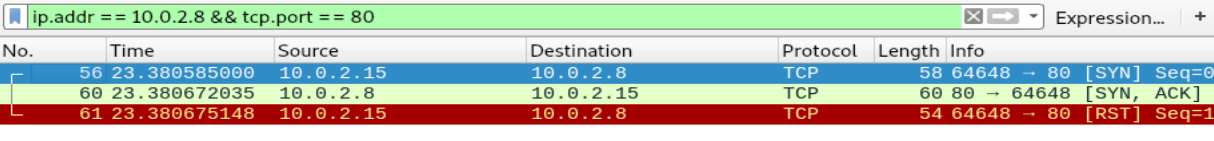
\includegraphics[width=1\textwidth]{oui/images/nmap/Wirebasique.PNG}
  \caption{Wireshark d'un scan de port 80}
  \label{fig:wirebasique}
\end{figure}

Dans le cas ci-dessus, l'attaquant est en 10.0.2.15 et la cible en 10.0.2.8. On se rend compte Nmap ne complète pas le Three-way Handshake et coupe brutalement la connexion via un RST TCP.
Ce scan est très rapide mais manque d'informations et est très visible sur le réseau... Il n'est pas forcément à privilégier.\\

 \textbf{Scan de version}\\

Si vous souhaitez obtenir des informations concerant le serveur de déployement du service afin de trouver des failles associées, il vous faudra utiliser l'option -sV de Nmap visualisable en \textbf{figure \ref{fig:sv}}.

\begin{figure}[htp!]
  \centering
  \setlength\figureheight{7cm}
  \setlength\figurewidth{9cm}
  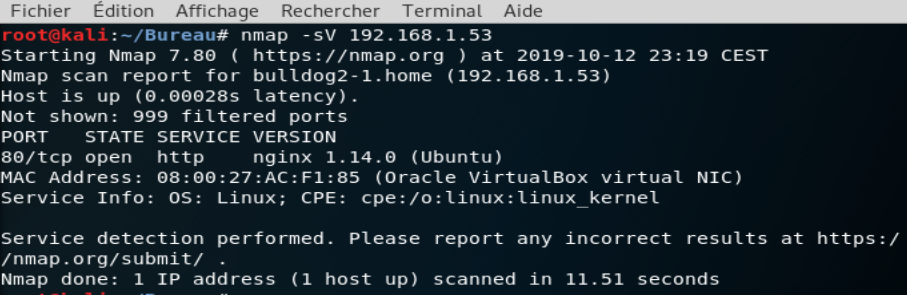
\includegraphics[width=0.8\textwidth]{oui/Ancien/imangeancien/Nmap/-sV.PNG}
  \caption{Scan de version}
  \label{fig:sv}
\end{figure}

\newpage
Ce scan affiche une nouvelle colonne qui contient les informations du service. Regardons ce qu'il se passe au niveau de Wireshark en \textbf{figure \ref{fig:svwire}}.

\begin{figure}[htp!]
  \centering
  \setlength\figureheight{7cm}
  \setlength\figurewidth{9cm}
  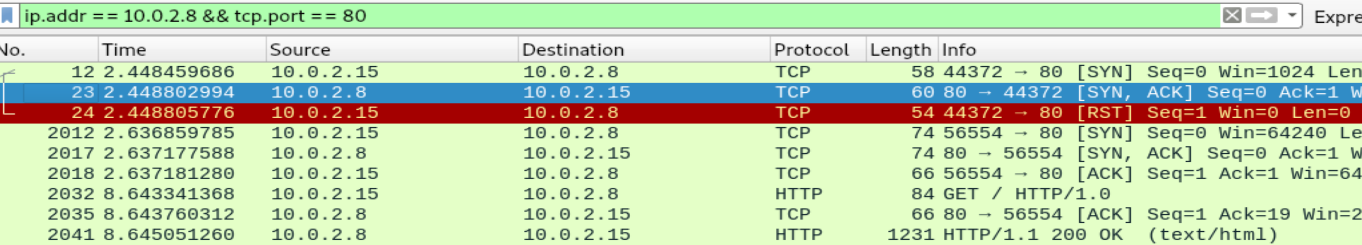
\includegraphics[width=1\textwidth]{oui/images/nmap/Wireversion.PNG}
  \caption{Obtention d'informations de version sous Wireshark}
  \label{fig:svwire}
\end{figure}

Dans un premier temps, nous retrouvons bien la demi-ouverture de port puis Nmap effectue le 3-way Handshake afin de se connecter au service qui est ici HTTP. Il va ensuite aller chercher dans son dictionnaire nmap-service-probes les requêtes à effectuer afin d'obtenir des informations. Dans notre cas, il va commencer par effectuer un GET et obtenir une réponse dans le HTTP/1.1 200 OK. Cela signifie que la page existe et que son retour est positif. Par exemple, si nous avions ouvert la réponse envoyée par la cible, nous aurions vu tout le contenu HTML de la page. Cette réponse est donc comparée à des expressions régulières présentes dans le fichier nmap-service-probes. Ce type de scan est donc plus approprié afin de trouver des failles. Cependant, il existe un moyen beaucoup plus complexe et complet qui est le scan via script.\\

 \textbf{Scan par script}\\

Dans le but d'obtenir des informations très précises, Nmap peut aussi s'éxecuter avec l'aide de scripts. Cette méthode s'appelle "Nmap Scripting Engine" ou NSE et s'appuie donc sur les mécanismes de Nmap et sur la légèreté des scripts Lua. Le langage Lua est très présent dans le monde du réseau comme par exemple dans Wireshark, dans les routeurs Cisco et d'autres. Nmap contient dans son répertoire près de 601 scripts regroupés sous 139 catégories. Il est donc tout à fait possible de créer un script et de l'excécuter avec Nmap. Cependant, nous allons nous baser sur un script déjà fait et qui exécute plusieurs scripts de différentes catégories afin d'obtenir des réponses précises et variées. Ce script est l'option par défault choisi par Nmap lors de la présence de l'argument -sC comme indiqué sur la \textbf{figure \ref{fig:nse}}.\\

\begin{figure}[t!]
  \centering
  \setlength\figureheight{7cm}
  \setlength\figurewidth{9cm}
  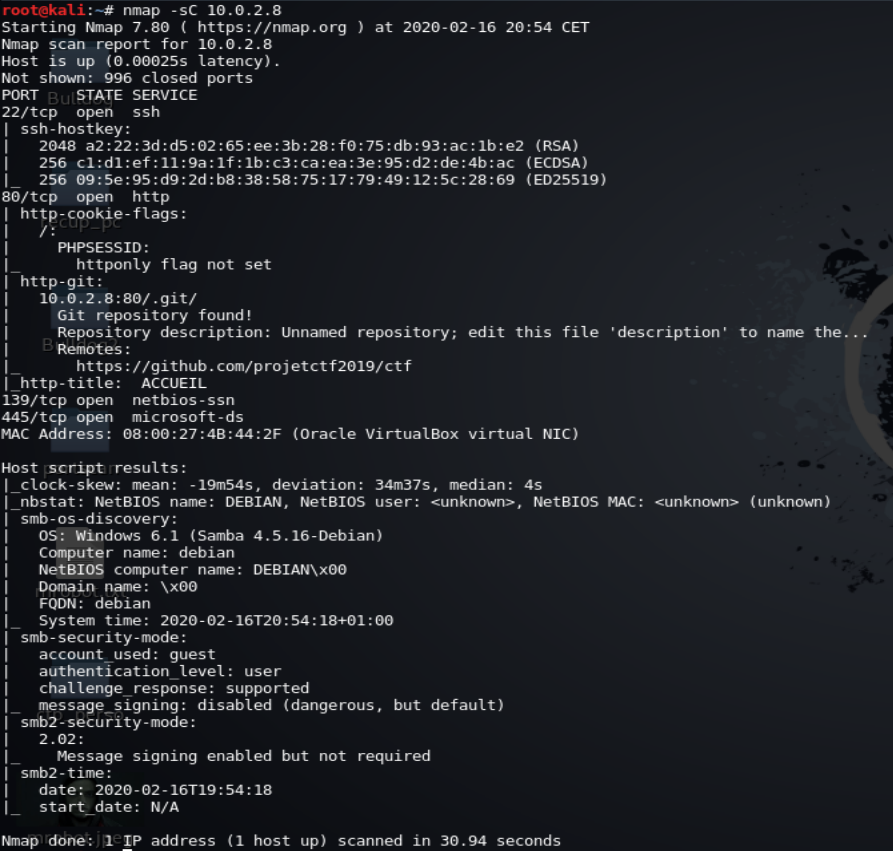
\includegraphics[width=0.8\textwidth]{oui/images/nmap/scriptscan.PNG}
  \caption{NSE par défaut}
  \label{fig:nse}
\end{figure}

On s'aperçoit que la quantité d'informations est très importante. Ce type de scan est le moyen ultime pour récupérer le plus d'informations possible. Il sera donc à privilégier lors d'un CTF.\\

\newpage

 \textbf{Devenir invisible}\\

Avoir des informations, c'est bien, mais les récupérer en étant discret, c'est mieux. En effet, si la machine cible n'était pas un CTF mais un cas réel d'attaque, il nous faudrait apprendre à ne pas être détécté. Il existe de multiples moyens que nous allons voir ici. Dans un premier temps, il faut savoir que Nmap utilise l'option -sS par défaut. Ce mode permet à Nmap de ne réaliser qu'une demi-ouverture de porte. Cet option est essentielle afin de ne pas être détecté trop vite. Ensuite, nous avons la possiblité d'usurper notre identité via un spoof MAC et IP comme on peut le voir sur la \textbf{figure \ref{fig:spoofip}}\\

\begin{figure}[]
  \centering
  \setlength\figureheight{7cm}
  \setlength\figurewidth{9cm}
  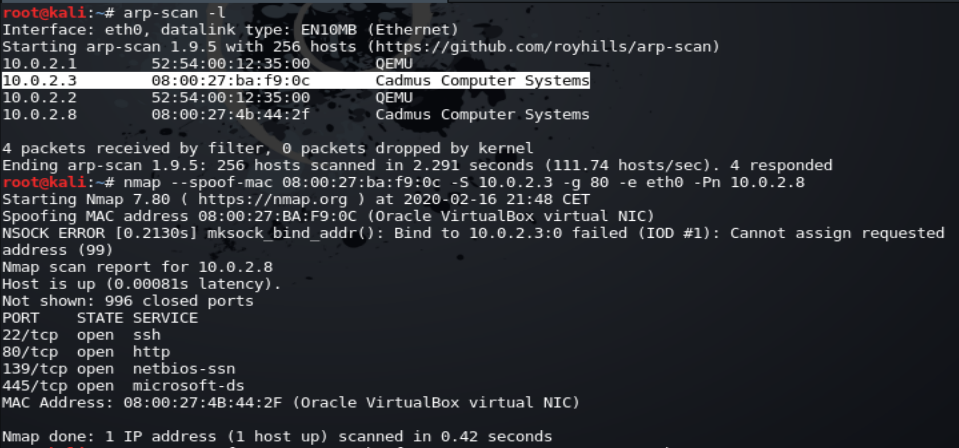
\includegraphics[width=1\textwidth]{oui/images/nmap/spoof.PNG}
  \caption{Spoof MAC et IP}
  \label{fig:spoofip}
\end{figure}

Cette méthode consiste à se faire passer pour quelqu'un du réseau via son adresse MAC et IP. L'option -g permet d'indiquer vers quel port de la machine usurpée Nmap va rediriger les échanges. L'option -e indique sur quelle interface réseau la machine attaquante va recevoir les informations telles que l'attaque "Man in the middle". Enfin, l'option -Pn n'est pas obligatoire mais elele est conseillée par Nmap en cas d'usurpation d'identité. En effet, cette option permet de bloquer le protocole ICMP et ainsi de ne pas être découvert.\\
%ça te va ?
La seconde méthode permet d'être moins visible vis à vis d'un firewall et de cibler les ports les plus connus tout en réduisant le temps de scan de ports. En moyenne, la durée d'un scan par défaut de Nmap est de 1 seconde. Il est possible de faire varier le temps d'un scan afin de faire baisser le nombre d'ouverture de ports par seconde en utilisant l'argument -Tx. Il est à notifier que le x est comprit entre 0 et 5 et que plus le x sera grand, plus le scan sera agressif. \\

\vspace{0.1cm}

Cependant, si on recherche à être discret et que l'on choisit un x valant 1 ou 0, le scan risque d'être très long... En effet, l'option -T1 réalise le scan en 30 secondes minimum tandis que le -T0 le réalise en 10 minutes ! La solution la plus adaptée est donc de cibler des ports stratégiques avec l'argument -p comme indiqué dans la \textbf{figure \ref{fig:port}}.\\



\begin{figure}[]
  \centering
  \setlength\figureheight{7cm}
  \setlength\figurewidth{9cm}
  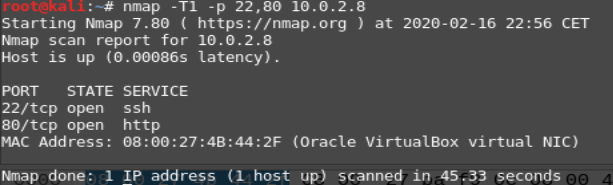
\includegraphics[width=1\textwidth]{oui/images/nmap/t1.PNG}
  \caption{Ciblage des ports}
  \label{fig:port}
\end{figure}

Nous avons donc compris dans cette partie que l'outil Nmap est essentiel lors d'une attaque et qu'il comporte énormément de fonctionnalités.

\section{Nikto}

\subsection{Présentation}
Nikto est un outil écrit en Perl permettant le scan de vulnérabiltés sur un serveur Web. Il permet de tester la sécurité de la configuration d'un serveur web (les options HTTP, les index, les potentielles failles XSS, injections SQL etc…).\\
Avant de montrer ce que peut réaliser Nikto, nous pouvons dans un premier temps revoir comment fonctionne une requête Web. Parmis les ports réservés, les serveurs Web utilise le port 80 pour HTTP et le port 443 pour l'HTTPS. Pour comprendre le fonctionnement, nous allons analyser un échange entre un client et un serveur sur la \textbf{figure \ref{fig:webdiag}}.\\



\begin{figure}[t]
  \centering
  \setlength\figureheight{7cm}
  \setlength\figurewidth{9cm}
  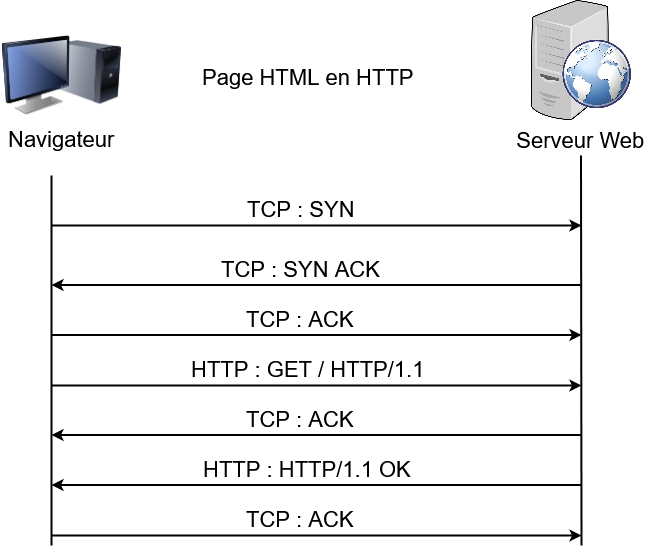
\includegraphics[width=0.7\textwidth]{oui/Ancien/imangeancien/Nikto/wEBDiagram.png}
  \caption{Échange entre un navigateur et un serveur Web}
  \label{fig:webdiag}
\end{figure}


Comme on peut le voir, le schéma sur la \textbf{figure \ref{fig:webdiag}}. ainsi que la capture wireshark en \textbf{figure \ref{fig:niktowire}} montrent l'échange minimal entre un navigateur et un serveur Web afin d'obtenir une page HTML via HTTP. Une page Web utilse le protocole TCP pour transmettre les paquets. En effet, lorsque nous chargeons une page Web, nous la voulons complète et sans erreurs. C'est pourquoi le protocole TCP existe. Au début de chaque trame TCP, il ya une synchronisation de la connexion avec le "3 way handshakes". Passons maintenant à la couche applicative : les envois HTTP sont directement émis par le navigateur et par le serveur Web. Ici, c'est notre navigateur qui fait une requête GET au serveur pour obtenir l'ensemble de la page Web voulue. Il existe plusieurs types de requêtes Web (GET, POST, HEAD, ...) mais seul le GET va nous intéresser car il est le plus utilisé. 

\begin{figure}[htp!]
  \centering
  \setlength\figureheight{7cm}
  \setlength\figurewidth{9cm}
  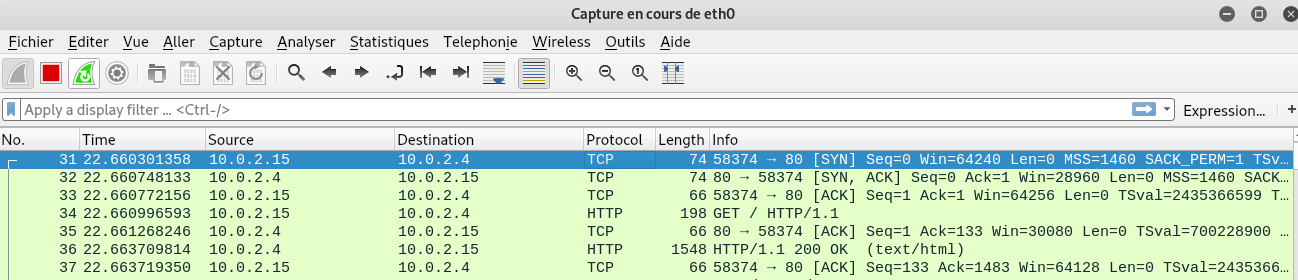
\includegraphics[width=0.7\textwidth]{oui/Ancien/imangeancien/Nikto/wireshark1.PNG}
  \caption{Capture Wireshark d'un scan nikto}
  \label{fig:niktowire}
\end{figure}


 Lors du scan, Nikto est capable de :\\
\textbf{- Vérifier} si la version du serveur est obsolète ainsi que les logiciels et     modules qui sont utilisés par ce dernier. \\   
\textbf{- Scanner} les répertoires, qui peuvent contenir des informations sensibles.\\
\textbf{- Tester} près de 6000 fichiers potentiellement vulnérables.\\
De plus, Nikto supporte les connexions SSL.


\newpage

\subsection{Utilisation de Nikto}

 Pour lancer un simple scan, il suffit de taper la commande :

\begin{figure}[htp!]
  \centering
  \setlength\figureheight{7cm}
  \setlength\figurewidth{9cm}
  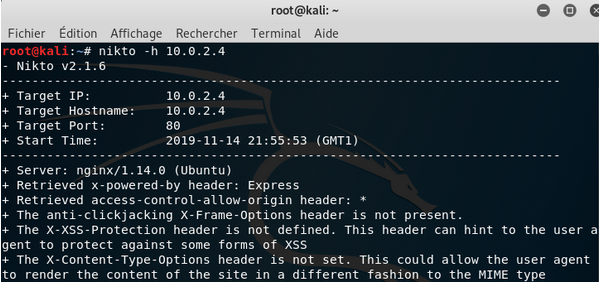
\includegraphics[width=0.7\textwidth]{oui/Ancien/imangeancien/Nikto/1.PNG}
  \caption{Scan simple}
  \label{fig:courbe-tikz}
\end{figure}

On peut remarquer grâce à cette capture wireshark que par défaut, Nikto scanne le port 80 :

\begin{figure}[htp!]
  \centering
  \setlength\figureheight{7cm}
  \setlength\figurewidth{9cm}
  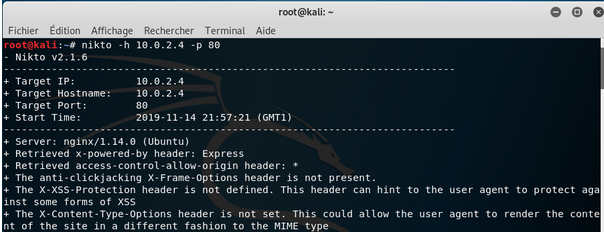
\includegraphics[width=0.7\textwidth]{oui/Ancien/imangeancien/Nikto/2.PNG}
  \caption{Scan d'un port}
  \label{fig:courbe-tikz}
\end{figure}

\begin{figure}[htp!]
  \centering
  \setlength\figureheight{7cm}
  \setlength\figurewidth{9cm}
  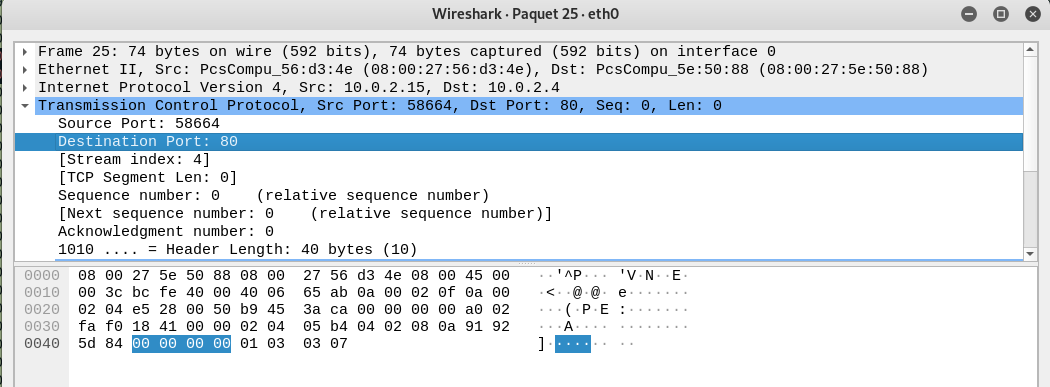
\includegraphics[width=0.7\textwidth]{oui/Ancien/imangeancien/Nikto/wireshark3.png}
  \caption{Mise en évidence du port scanné par défaut par la commande nikto}
  \label{fig:courbe-tikz}
\end{figure}

\newpage

Afin de scanner un port précis, il faut ajouter l'argument \textbf{-p}: 

\begin{figure}[htp!]
  \centering
  \setlength\figureheight{7cm}
  \setlength\figurewidth{9cm}
  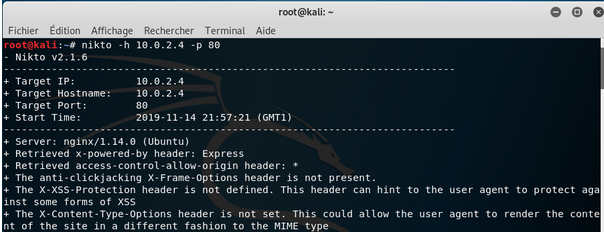
\includegraphics[width=0.8\textwidth]{oui/Ancien/imangeancien/Nikto/2.PNG}
  \caption{Scan d'un port}
  \label{fig:courbe-tikz}
\end{figure}

Dans cette capture, nous venons de scanner l'IP sur le port 80 (http). Il également possible de cibler plusieurs ports en même temps:


\begin{figure}[htp!]
  \centering
  \setlength\figureheight{7cm}
  \setlength\figurewidth{9cm}
  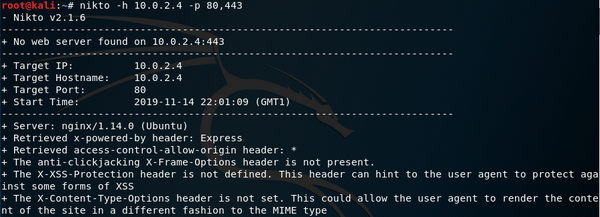
\includegraphics[width=0.8\textwidth]{oui/Ancien/imangeancien/Nikto/3.PNG}
  \caption{Scan de plusieurs ports}
  \label{fig:courbe-tikz}
\end{figure}

A partir de ces captures, on peut en déduire que Nikto est capable de nous fournir le logiciel qui permet de faire fonctionner le serveur web, sa version et également le système d'exploitation utilisé. En effet, toutes ces informations sont comprises dans l'entête des réponses HTTP du serveur. Nikto est également capable de vérifier les mauvaises configurations de services ou de programmes mal sécurisé. Cet outil propose également des plugins permettant la recherche d'autres vulnérabilités ou de fichier pouvant être intéressant dans un CTF tel que le fichier \textbf{robots.txt}. Ce fichier permet le référencement d'un site WEB par les robots de Google. Cependant, l'administrateur peut empêcher le scan de certains répertoires par les robots en précisant dans ce fichier quelques paramètres. Ainsi, grâce à cela, un attaquant peut utiliser ce fichier pour découvrir des répertoires que l'administrateur aurait voulu cacher.

\begin{figure}[htp!]
  \centering
  \setlength\figureheight{7cm}
  \setlength\figurewidth{9cm}
  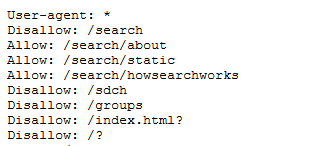
\includegraphics[width=0.5\textwidth]{oui/Ancien/imangeancien/Nikto/robots.PNG}
  \caption{Extrait fichier robots.txt}
  \label{fig:courbe-tikz}
\end{figure}

 On comprend à travers cette capture que le paramètre \textbf{Disallow} empêche le scan de ce répertoire.\\

\subsection{Gagner en discrétion pendant les scans}
Une méthode pour gagner en discrétion pendant l'attaque serait d'effectuer un scan par intervalle. En effet, si on effectue un scan toutes les 10 secondes, cela paraîtra moins suspect qu'un scan toutes les 1ms. Cela est possible en ajoutant l'option \textbf{-Pause 10} en argument :

\begin{figure}[htp!]
  \centering
  \setlength\figureheight{7cm}
  \setlength\figurewidth{9cm}
  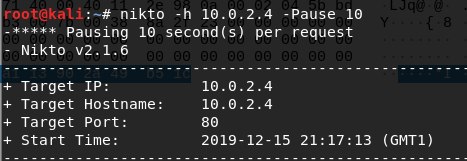
\includegraphics[width=0.8\textwidth]{oui/Ancien/imangeancien/Nikto/nikto9.png}
  \caption{Ajout de l'argument Pause}
  \label{fig:courbe-tikz}
\end{figure}

Voici une capture wireshark de ce scan avec l'ajout de l'argument :

\begin{figure}[htp!]
  \centering
  \setlength\figureheight{7cm}
  \setlength\figurewidth{9cm}
  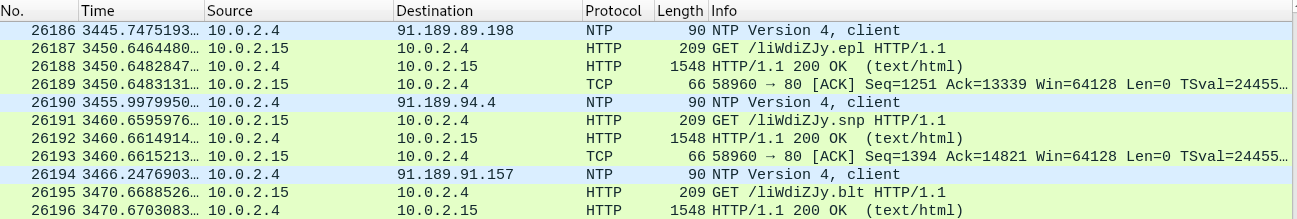
\includegraphics[width=1\textwidth]{oui/Ancien/imangeancien/Nikto/wireshark4.PNG}
  \caption{Capture wireshark du scan avec l'otpion de pause}
  \label{fig:courbe-tikz}
\end{figure}

 On remarque l'utilisation du protocole NTP (Network Time Protocol) qui permet ici de mettre en place le temps de pause.
\newpage

\section{Dirb/Dirbuster}

Après avoir réalisé un scan via Nmap et repéré qu'un serveur Web est activé, Dirb sera là pour vous guider à travers les pages car il est un scanneur de contenu Web. Son but est de trouver l’existence d’objets web, qu’ils soient cachés ou non.
Son fonctionnement réside en la lancée d’une attaque par dictionnaire contre un serveur web et d’en analyser la réponse. \\
Cependant, il existe une différence entre une attaque par dictionnaire et une attaque par bruteforce pure.\\
Une attaque par dictionnaire est une attaque que l’on utilise dans la cryptanalyse (technique de déduction d’un texte en clair par rapport à un texte chiffré sans la clé de chiffrement) pour justement trouver un mot de passe ou une clé de chiffrement. 
Son fonctionnement consiste à tester une liste donnée de mots de passe potentiels, un par un, en espérant que le mot de passe de chiffrement soit l’un deux. 
Cette technique ne marche donc pas systématiquement et il faut une énorme liste de mots de passe et du temps pour qu’elle soit efficace. L'intérêt d'installer des dictionnaires supplémentaires serait utile dans les cas de mots de passe très complexes.
C’est d’ailleurs à cause de ce genre d’attaque que l’on conseille de mettre des mots de passe compliqués, car ceux courants sont bien plus simples à trouver avec ce genre d’attaque. 

\subsection{Création de dictionnaires et utilisation de Dirb}

Comme nous l'avons plus haut, Dirb se base sur un dicitonnaire afin de réaliser son scan. Nous avons donc quatre possibilités :

\begin{itemize}
    \item \textbf{Créer un dictionnaire à partir d'une page Web}
    \item \textbf{Créer un dictionnaire sous forme de pattern}
    \item \textbf{Créer un dictionnaire aléatoire}
    \item \textbf{Utiliser un dictionnaire présent dans le répertoire de Dirb}\\
\end{itemize}

 \textbf{Créer un dictionnaire à partir d'une page Web}\\

Cette méthode est plus utilisée avec l'outil John que Dirb mais il est important de l'expliquer ici. En effet, utiliser des mots présents sur une page Web peut être intéressant dans le cas où nous avons un mot de passe hasher à découvrir. Il vous faudra donc télécharger la page Web en question via un wget et réaliser la commande suivante :

\begin{figure}[htp!]
  \centering
  \setlength\figureheight{7cm}
  \setlength\figurewidth{9cm}
  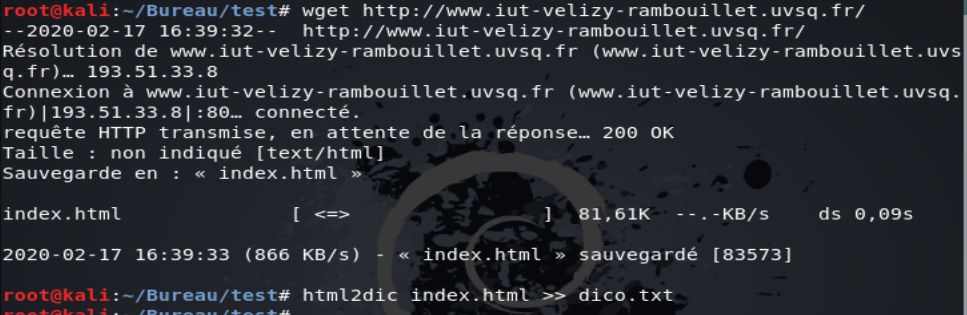
\includegraphics[width=1\textwidth]{oui/images/Dirb/html2dic.PNG}
  \caption{Html2dic}
  \label{fig:courbe-tikz}
\end{figure}

\newpage
C'est ainsi que nous pouvons créer un premier dictionnaire assez rapidement.\\

 \textbf{Créer un dictionnaire sous forme de pattern}\\

Lorsque que l'on connaît une partie du mot ou page que l'on recherche, utiliser un pattern peut être la solution. Un pattern est une forme commune qui va varier sur une partie pré-définie. Gendict est l'outil de création de dictionnaire avec pattern que nous allons utiliser ici. Il vous faudra cependant l'installer via le paquet "icu-devtools". Voici son utilisation :

\begin{figure}[htp!]
  \centering
  \setlength\figureheight{7cm}
  \setlength\figurewidth{9cm}
  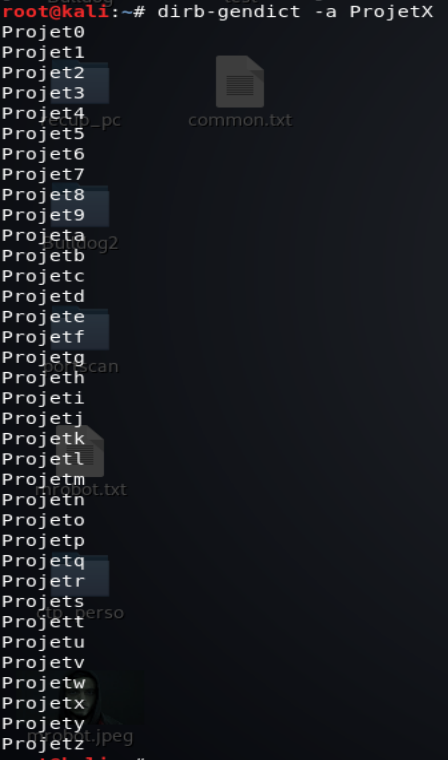
\includegraphics[width=0.34\textwidth]{oui/images/Dirb/gendict.PNG}
  \caption{Gendict -a}
  \label{fig:courbe-tikz}
\end{figure}

On comprend ici que le X sera la variable du pattern. Il est donc tout à fait possible de créer un dictionnaire sans pattern en mettant un nombre de X correspondant à la taille recherchée comme ceci :

\begin{figure}[htp!]
  \centering
  \setlength\figureheight{7cm}
  \setlength\figurewidth{9cm}
  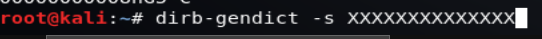
\includegraphics[width=0.9\textwidth]{oui/images/Dirb/dicoaleatoire.PNG}
  \caption{Gendict -s}
  \label{fig:courbe-tikz}
\end{figure}

L'option -s permet d'obtenir aussi les majuscules. Les deux principaux défauts de Gendict en tant que créateur de dictionnaires aléatoires sont les suivants :

\begin{itemize}
    \item \textbf{Le manque de caractères spéciaux}
    \item \textbf{La taille est fixe en fonction du nombre de X}
\end{itemize}

C'est pour cette raison qu'il existe un autre outil spécialisé dans la conception de dictionnaires aléatoires.\\

 \textbf{Créer un dictionnaire aléatoire}\\

L'outil que nous considérons comme le plus efficace en terme de création de dictionnaires aléatoires est l'outil Crunch. Ce dernier, en plus de réaliser du pattern, complète les défauts de Gendict. Nous allons vous présenter la manière pour réaliser le dictionnaire le plus complet possible de manière aléatoire. Tout d'abord, Crunch se base sur un dictionnaire se nommant "charset.lst". Vous y retrouverez les séries de caractères que vous pouvez choisir pour réaliser votre dictionnaire. Dans notre cas, nous avons choisis d'utiliser la série mixalpha-numeric-all-space et nous l'avons enregistré dans un fichier dico.txt comme ci-dessous :

\begin{figure}[htp!]
  \centering
  \setlength\figureheight{7cm}
  \setlength\figurewidth{9cm}
  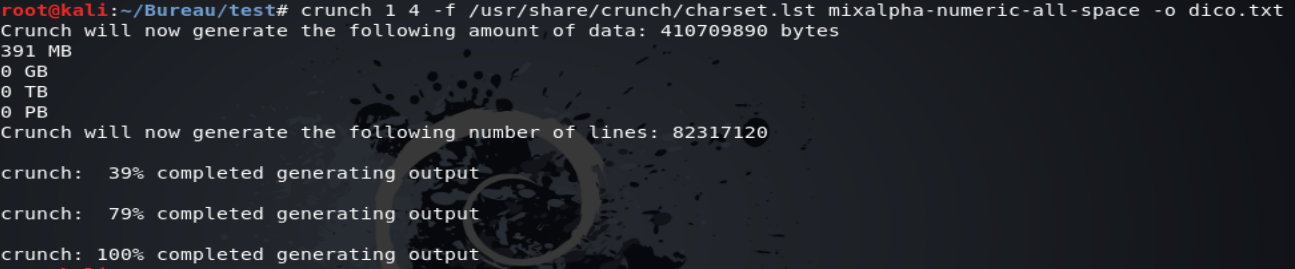
\includegraphics[width=1\textwidth]{oui/images/Dirb/crunch.PNG}
  \caption{Crunch}
  \label{fig:courbe-tikz}
\end{figure}

Comme vous pouvez le voir au début de la commande, nous avons spécifié que les mots devaient être générés entre 1 et 4 caractères et l'outil nous annonce que le dictionnaire fera 391 MB ! Pour information, les sites Web demandent en général un mot de passe avec au minimum 8 caractères. Je vous laisse donc lire la taille du dictionnaire si l'on souhaitait des mots de 1 à  8 caractères :

\begin{figure}[htp!]
  \centering
  \setlength\figureheight{7cm}
  \setlength\figurewidth{9cm}
  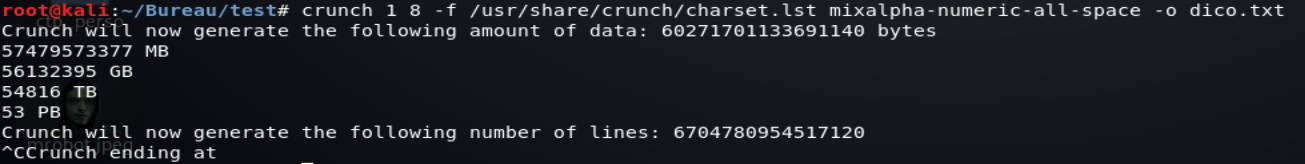
\includegraphics[width=1\textwidth]{oui/images/Dirb/crunch2.PNG}
  \caption{Crunch}
  \label{fig:courbe-tikz}
\end{figure}

Il est donc certain que cet outil vous permettra d'avoir un dictionnaire le plus complet au monde à la seule condition d'avoir une très grosse station de stockage... Heureusement que les concepteurs de Dirb ont pensé à ce détail et nous ont fourni des dictionnaires par défaut.\\

 \textbf{Utiliser un dictionnaire présent dans le répertoire de Dirb}\\

Comme nous l'avons vu précedemment, créer un dictionnaire peut vite devenir fastidieux. C'est pour cette raison que nous allons nous baser sur les dictionnaires présents dans le répertoire de Dirb. Il en existe plusieurs mais ici, nous allons utiliser le dictionnaire common.txt :

\begin{figure}[htp!]
  \centering
  \setlength\figureheight{7cm}
  \setlength\figurewidth{9cm}
  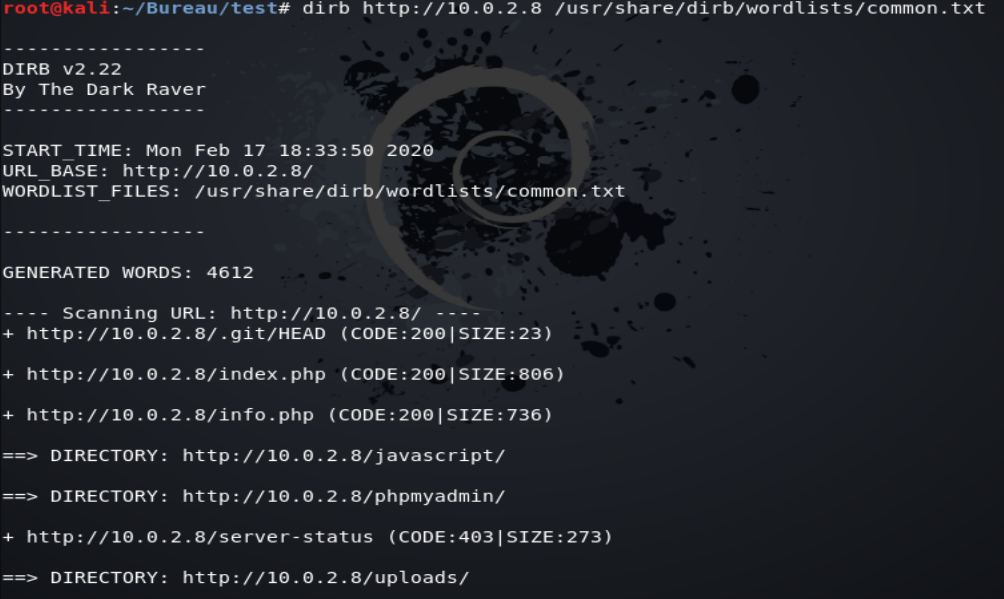
\includegraphics[width=1\textwidth]{oui/images/Dirb/dirb.PNG}
  \caption{Utilisation de Dirb}
  \label{fig:courbe-tikz}
\end{figure}

Encore une fois, l'utilisation d'un dictionnaire est très personnel. Il vous suffira donc de changer le dictionnaire et de lancer la commande afin d'obtenir un résultat. Comme vos pouvez le voir sur la capture d'écran ci-dessus, Dirb nous donne des pages cachées que nous n'aurions pas forcément trouvé tout seul. Cet outil est donc essentiel lors d'un pentest Web.

\subsection{Comparaison entre Dirb et Dirbuster}

Pour ceux qui préfèrent les interfaces graphiques aux lignes de commandes, il existe l'équivalent de Dirb en GUI (Graphical User Interface) qui se nomme Dirbuster.

Ce dernier permet, lui aussi, d’attaquer un site par dictionnaire. Il suffit de rentrer l'adresse IP du site ainsi que le répertoire où est stocké la liste de mots visible en \textbf{figure \ref{fig:dirbuster}}. 

\begin{figure}[htp!]
  \centering
  \setlength\figureheight{7cm}
  \setlength\figurewidth{9cm}
  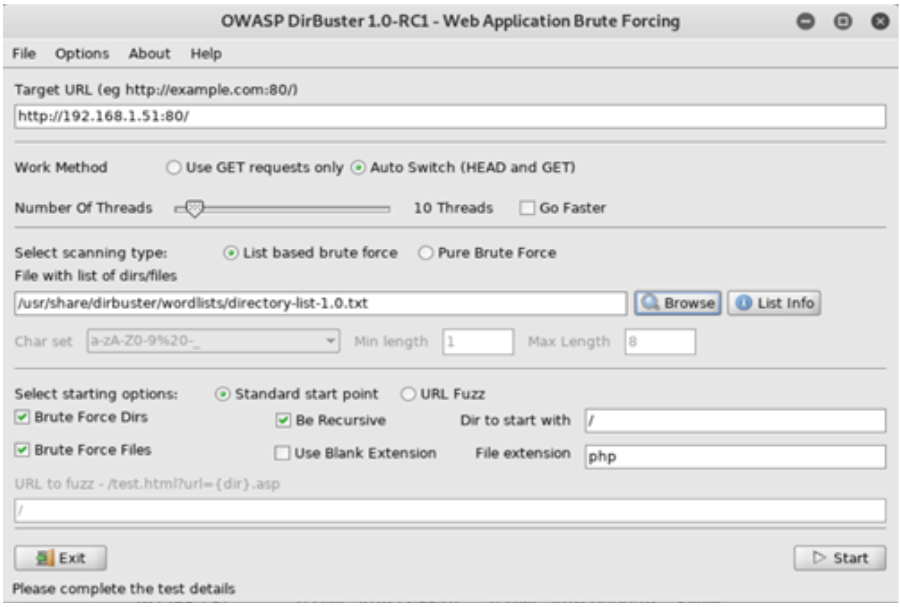
\includegraphics[width=0.8\textwidth]{oui/Ancien/imangeancien/dirb1.PNG}
  \caption{Dirbuster}
  \label{fig:dirbuster}
\end{figure}

L’utilisation de Dirb et Dirbuster est fondamentalement la même, mais ils ont chacun leurs avantages. 

Tout d’abord pour la question de rapidité, Dirb est en single-threading alors que Dirbuster est en multi-threading. \\
La différence entre single et multi est qu’en single, on ne peut exécuter les tâches qu’une par une de la manière suivante : 
\begin{center}
   \begin{figure}[htp!]
  \centering
  \setlength\figureheight{7cm}
  \setlength\figurewidth{9cm}
  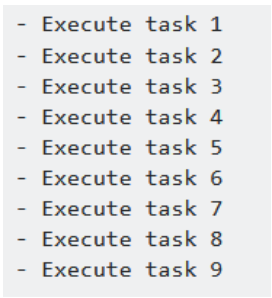
\includegraphics[width=0.25\textwidth]{oui/Ancien/imangeancien/dirb3.PNG}
  \caption{Single-threading}
  \label{fig:courbe-tikz}
\end{figure} 
\end{center}

 Alors que le multi-threading, lui, permet de faire plusieurs tâches en même temps en ordonnant les tâches en plusieurs threads, de la manière suivante : 
\begin{center}
    \textbf{Thread1}:\\
       \begin{figure}[htp!]
  \centering
  \setlength\figureheight{7cm}
  \setlength\figurewidth{9cm}
  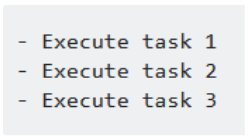
\includegraphics[width=0.25\textwidth]{oui/Ancien/imangeancien/dirb4.PNG}
  \label{fig:courbe-tikz}
\end{figure}
\textbf{Thread2}:\\
       \begin{figure}[htp!]
  \centering
  \setlength\figureheight{7cm}
  \setlength\figurewidth{9cm}
  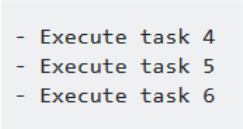
\includegraphics[width=0.25\textwidth]{oui/Ancien/imangeancien/dirb5.PNG}
  \label{fig:courbe-tikz}
\end{figure}

\textbf{Thread3}:\\
       \begin{figure}[htp!]
  \centering
  \setlength\figureheight{7cm}
  \setlength\figurewidth{9cm}
  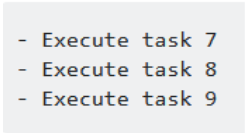
\includegraphics[width=0.25\textwidth]{oui/Ancien/imangeancien/dirb6.PNG}
  \caption{Multi-threading}
  \label{fig:courbe-tikz}
\end{figure}
\end{center}
Il faut noter que la différence ne se voit qu’avec des processeurs multi-coeurs, qui peuvent faire plusieurs tâches à la fois. \\
Donc pour la rapidité d’exécution, si nous avons un bon processeur, Dirbuster surpasse largement Dirb.
Seulement, Dirbuster demande toujours une interaction graphique, alors que Dirb, étant une CLI (Command Line Interface), permet l’automatisation, donc on perd certes du temps sur l’exécution des tâches mais on gagne du temps sur le reste.\\
Certes, Dirb vous fournira les fichiers tel que robots.txt mais ne fournira pas le code source des pages. N'hésitez pas à les observer car elles contiennent beaucoup d'informations. 